\section{On-the-fly-programming}

Alright. We are in the examples directory and you want to run ChucK from the terminal for the first time. To do so, type: 

In this case, ChucK will run whatever is in {\bf moe.ck}. You can, of course, replace {\bf moe.ck} with the name of another ChucK file. If this script is a just a loop that never ends then we need to stop ChucK eventually. Simple press CONTROL-C (hold control and press c). This is the kill process key in the terminal. 
Where is the ChucK power that was promised to you? You can add multiple copies of the same script if you like: 

Again, if any of these scripts will go on forever then you have to use the magic CONTROL-C to halt ChucK. Why would you do that? If the script has some random number generators or something like that then you end up with some nice ChucK chaos! Give it a try. 

Some first things to try to test the concurrency (running multiple ChucK files in parallel) are moe, larry, and curly. To listen to {\bf moe.ck}, {\bf larry.ck}, or {\bf curly.ck} together type: They are written to go in and out of phase with each other. 

Also try the improved versions of our little friends: 

Digging Deeper 

Now lets roll up our sleeves a little bit and see some real ChucK power! We are going to run two window ChucK, and on-the-fly! 

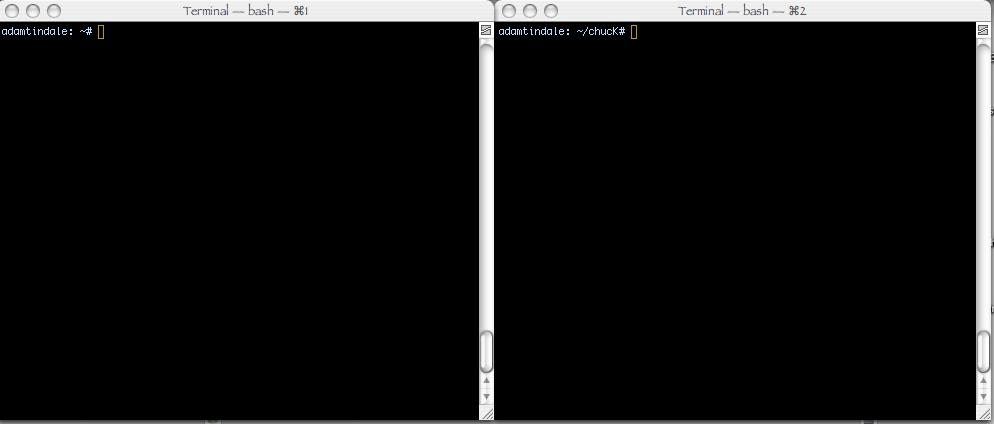
\includegraphics[width=\textwidth]{images/2term}

(on xp do such and such on OSX do such and such on linux do such and such)
Here is what you do: open another terminal window just like this one. Click on run in the Start Menu and type cmd in it; just like before. In this new window type chuck --loop    


This will start ChucK running. ChucK is now waiting for something to do. Go back to your original window where you are in your ChucK home. Be careful. If you type chuck test1.ck you will start a second ChucK running test1.ck. What we want to do is add a script to the ChucK that we set running in our second window. We will use the + operator to add a script to our ChucK and the - operator to remove a script. 

What hapenned? That is the power. We added test1.ck. It was added as the first shred in our ChucK. Since we knew it was shred 1 we removed it by typing chuck - 1. Great. Next we added three copies of the same script! Isn't that cool? You can also do this chuck + test1.ck test1.ck test1.ck How do you keep track of shreds? 

You can ask ChucK how he is doing by typing chuck --status The shortcut is chuck \^ ChucK will answer in the other window where we left him running. He will tell you what shreds there are and what their id numbers are. He will also tell you how long he has been running. Great. 

When you have had enough of ChucK you can go to the other window and use your fancy CONTROL-C trick or you can type chuck --kill in your original window.   


 chuck + test1.ck    chuck - 1     chuck + test1.ck    chuck + test1.ck    chuck + test1.ck    chuck - 1 2 3

chuck moe.ck    chuck moe.ck moe.ck    chuck moe.ck larry.ck curly.ck    chuck moe++.ck larry++.ck curly++.ck